\usetikzlibrary{fit, positioning, shapes.geometric, backgrounds}
\begin{figure*}
\centering
\begin{minipage}[t]{.32\textwidth}
\begin{subfigure}{.9\textwidth}
\centering
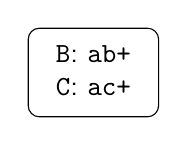
\begin{tikzpicture}[
box/.style={draw, rounded corners, minimum width=7cm, font=\sffamily},
]
    \node[box, inner sep=4pt, minimum height=0pt, minimum width=0pt] (terminals) {
    \begin{tabular}{l}
      \texttt{B}: \texttt{ab+}\\
      \texttt{C}: \texttt{ac+}
    \end{tabular}
    };
\end{tikzpicture}
\caption{Terminals and regular expressions.}
\label{fig:overview_terminals}
\end{subfigure}

\begin{subfigure}{.8\textwidth}
\centering
\begin{tikzpicture}[
    shorten >=1pt,
    node distance=2.0cm and 1.3cm,
    on grid,
    auto,
    scale=1.0,
    every state/.style={minimum size=0.8cm}
] 
   \node[state,initial,initial text={}] (q_0)   {$q_0$}; 
   \node[state] (q_1) [right=of q_0] {$q_1$}; 
   \node[state, accepting] (q_2) [right=of q_1, yshift=20pt] {$q^{\texttt{B}}_2$}; 
   \node[state, accepting] (q_3) [right=of q_1, yshift=-20pt] {$q^{\texttt{C}}_3$};

    \path[->] 
    (q_0) edge node {\texttt{a}} (q_1)

    (q_1) edge node[pos=0.5] {\texttt{b}} (q_2) 
          edge node[swap, pos=0.5] {\texttt{c}} (q_3) 

    (q_2) edge [loop right] node[pos=0.15, above] {
            \texttt{b}
            } ()


    (q_3) edge [loop right] node[pos=0.15, above] {\texttt{c}} ()

;
\end{tikzpicture}
\caption{Lexing automaton obtained from terminal definitions in \autoref{fig:overview_terminals}.}
\label{fig:overview_nfa}
\end{subfigure}
\end{minipage}
%
\begin{minipage}[t]{.48\textwidth}
\begin{subfigure}{.9\textwidth}
\centering
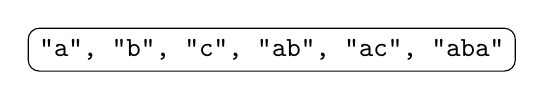
\begin{tikzpicture}[
box/.style={draw, rounded corners, minimum width=7cm, font=\sffamily},
]
    % LLM Vocab box
    \node[box, inner sep=4pt, minimum height=0pt, minimum width=0pt] {
      \texttt{"a", "b", "c", "ab", "ac", "aba"}
    };
\end{tikzpicture}
\caption{Subword vocabulary for the LLM.}
\label{fig:overview_vocab}
\end{subfigure}


\begin{subfigure}{.9\textwidth}
\centering
\vspace{32pt}
\resizebox{7cm}{!}{
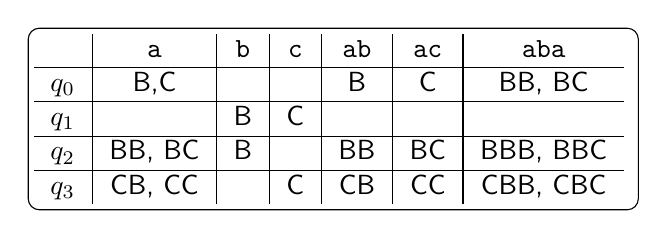
\begin{tikzpicture}[
    tablebox/.style={draw, rounded corners, align=center, font=\sffamily, inner sep=2pt}
]
    \node[tablebox] (lookup) {
      \begin{tabular}{c|c|c|c|c|c|c}
      {} & \texttt{a} & \texttt{b} & \texttt{c} & \texttt{ab} & \texttt{ac} & \texttt{aba} \\ \hline
      $q_0$ &  B,C & $\varnothing$ & $\varnothing$ & B   &  C   &  BB, BC   \\ \hline
      $q_1$ & $\varnothing$ & B & C & $\varnothing$   &  $\varnothing$  &  $\varnothing$   \\ \hline
      $q_2$ &  BB, BC & B & $\varnothing$ & BB   & BC   &  BBB, BBC   \\ \hline
      $q_3$ &  CB, CC & $\varnothing$ & C & CB   &   CC   & CBB, CBC    
      \end{tabular}
    };
\end{tikzpicture}
}
\caption{\Table computed from lexing automaton (\autoref{fig:overview_nfa}) and subword vocabulary (\autoref{fig:overview_vocab}).}
\label{fig:overview_table}
\end{subfigure}
\end{minipage}
%
\begin{minipage}[t]{.19\textwidth}
\begin{subfigure}{.9\textwidth}
\centering
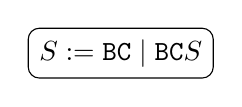
\begin{tikzpicture}[
box/.style={draw, rounded corners, minimum width=7cm, font=\sffamily},
]
    \node[box, inner sep=4pt, minimum height=0pt, minimum width=0pt] {
        $S := \texttt{BC} \mid \texttt{BC}S$
    };
\end{tikzpicture}
\caption{Grammar $\grammar_{\texttt{BC}}$.}
\label{fig:overview_cfg}
\end{subfigure}

\begin{subfigure}{.9\textwidth}
\centering
\begin{tikzpicture}[
    shorten >=1pt,    
    every state/.style={minimum size=0.8cm},
    node distance=0.5cm and 1cm,
    box/.style={draw, rounded corners, font=\sffamily},
    tablebox/.style={draw, rounded corners, align=center, font=\sffamily},
    labelbox/.style={font=\bfseries\sffamily},
    every node/.style={outer sep=2pt}
]
   \node[state,initial above,initial text={}] (q_0) []  {$S_0$}; 
   \node[state] (q_1) [below=of q_0, xshift=-30pt] {$S_1$}; 
   \node[state,accepting] (q_2) [below=of q_0, xshift=30pt] {$S_2$}; 
   % \node[state] (q_4) [below=of q_3] {$q^{(}_4$};
   % \node[state] (q_5) [below=of q_4] {$q^{)}_5$};
    \path[->] 
    (q_0) edge node[above=10pt, pos=0.8] {\texttt{B}} (q_1)
    (q_1) edge node[above] {\texttt{C}} (q_2)
    (q_2) edge node[above=10pt, pos=0.2] {$\epsilon$} (q_0)
;
\end{tikzpicture}    
\caption{Automaton for  the grammar in \autoref{fig:overview_cfg}.}
\label{fig:overview_pda}
\end{subfigure}
\end{minipage}
\caption{Illustrative example of the approach implemented in \name.}
\label{fig:overview}
\end{figure*}